
%% bare_conf.tex
%% V1.4b
%% 2015/08/26
%% by Michael Shell
%% See:
%% http://www.michaelshell.org/
%% for current contact information.
%%
%% This is a skeleton file demonstrating the use of IEEEtran.cls
%% (requires IEEEtran.cls version 1.8b or later) with an IEEE
%% conference paper.
%%
%% Support sites:
%% http://www.michaelshell.org/tex/ieeetran/
%% http://www.ctan.org/pkg/ieeetran
%% and
%% http://www.ieee.org/

%%*************************************************************************
%% Legal Notice:
%% This code is offered as-is without any warranty either expressed or
%% implied; without even the implied warranty of MERCHANTABILITY or
	%% FITNESS FOR A PARTICULAR PURPOSE! 
%% User assumes all risk.
%% In no event shall the IEEE or any contributor to this code be liable for
%% any damages or losses, including, but not limited to, incidental,
%% consequential, or any other damages, resulting from the use or misuse
%% of any information contained here.
%%
%% All comments are the opinions of their respective authors and are not
%% necessarily endorsed by the IEEE.
%%
%% This work is distributed under the LaTeX Project Public License (LPPL)
%% ( http://www.latex-project.org/ ) version 1.3, and may be freely used,
%% distributed and modified. A copy of the LPPL, version 1.3, is included
%% in the base LaTeX documentation of all distributions of LaTeX released
%% 2003/12/01 or later.
%% Retain all contribution notices and credits.
%% ** Modified files should be clearly indicated as such, including  **
%% ** renaming them and changing author support contact information. **
%%*************************************************************************


% *** Authors should verify (and, if needed, correct) their LaTeX system  ***
% *** with the testflow diagnostic prior to trusting their LaTeX platform ***
% *** with production work. The IEEE's font choices and paper sizes can   ***
% *** trigger bugs that do not appear when using other class files.       ***                          ***
% The testflow support page is at:
% http://www.michaelshell.org/tex/testflow/



\documentclass[conference]{IEEEtran}
% Some Computer Society conferences also require the compsoc mode option,
% but others use the standard conference format.
%
% If IEEEtran.cls has not been installed into the LaTeX system files,
% manually specify the path to it like:
% \documentclass[conference]{../sty/IEEEtran}


% correct bad hyphenation here
\hyphenation{op-tical net-works semi-conduc-tor}


\usepackage{graphicx} % Required for the inclusion of images

\begin{document}
%
% paper title
% Titles are generally capitalized except for words such as a, an, and, as,
% at, but, by, for, in, nor, of, on, or, the, to and up, which are usually
% not capitalized unless they are the first or last word of the title.
% Linebreaks \\ can be used within to get better formatting as desired.
% Do not put math or special symbols in the title.
\title{Literature Survey of SHA-256 Hardware implementations for ECSE 682 project}


% author names and affiliations
% use a multiple column layout for up to three different
% affiliations
\author{\IEEEauthorblockN{Shabbir Hussain}
\IEEEauthorblockA{Dept. of Computer Engieering, 
McGill University\\
Montreal, Quebec\\
Email: shabbir.hussain@mail.mcgill.ca}
}

% make the title area
\maketitle

% As a general rule, do not put math, special symbols or citations
% in the abstract
\begin{abstract}
SHA-256 is a cryptographic one way hashing algorithm used to verify the authenticity of files and messages. It is a NIST standard used in many protocols such as SSH, PGP, IPSec and HMAC. Hardware implementations of the SHA-256 algorithm have been proposed in the literature to reduce the power and performance footprint of cryptographic calculations on General Purpose Processors (GPP). These implementations use techniques such as Loop unrolling, pipelining, retiming to speed up hashing and can achieve performance boosts up to 150x, with throughput of 11GBps and power as low as 46mW.
\end{abstract}

\IEEEpeerreviewmaketitle



\section{Introduction} \label{introduction}
Cryptography is often known as a practice to send secret messages. While encrypting and decrypting messages are an important part of keeping secrets, so too is the method of verifying that message content is unaltered from sender to receiver. One of the methods employed to make sure that a message remains unmodified in transit is called a Message Authentication Code (MAC). These codes are computed based on the message contents and a shared secret key between sender and receiver. A MAC provides message integrity because an imposter can not feasibly create a false message and MAC pair or modify the contents of an existing message that will trick the receiver into believing that the messages were authored by the true sender \cite{schneier}. This is because the generation and verification of a MAC involves using a cryptographically secure hash function such as the SHA-256 algorithm. The SHA-256 algorithm is a NIST standard that is part of a family hash functions called the SHA2 family. These functions take as input an arbitrary length string of bits and compute fixed length string of bits called the Digest Message (DM). These functions are one way functions with a low chance of collisions. Changing 1 bit of the input dramatically changes the output making it very difficult to guess the input based on the output. This property is what gives it its relevance in the field of cryptography. The only way to compute the input a DM is to guess and as of writing this paper there no known attacks on the SHA-256 to speed up this process. Given a 256 bit DM it would take a modern computer several years to find the corresponding input. This is because cryptographic functions are slow in general.\\ Computing a MAC for every message adds a performance and power penalty. IPSec’s performance bottleneck is the HMAC mechanism which
is responsible for authenticating the transmitted data \cite{michail}. VLSI is literature is rich in solutions that offload the has computation to hardware to quickly compute hashes with a low power and area foot print. This paper surveys three recent designs that implement the SHA-256 algorithm in hardware. 

The paper will be divided as follows. Section \ref{sha256} will present the sha256 algorithm. Section \ref{sha2fam} will discuss the design by Sklavos et al. Section \ref{cesha} will explain the design by Chaves et al. Section \ref{Explsha} will explain the design by Michail et al. Finally, section \ref{Conclusion} will have concluding thoughts about all three implementations and an outlook into the future work that can be done.

\section{SHA-256 algorithm} \label{sha256}
The SHA-256 algorithm takes in a bit string of a maximum size of $2^{64}$ bits and outputs a 256-bit output called the Digest Message (DM) \cite{nist}. The SHA-256 algorithm can be divided into three steps.
\begin{enumerate}
  \item Padding
  \item Data Initialisation
  \item Round Hashing
\end{enumerate}

During the Padding step, the input message is subdivided into 512 bit blocks. The last block is padded to a multiple of 512 bits. At the end of the contents of the last block a 1 bit is placed followed by zeroes. The last 64 bits of that block are used to store the message length. Figure \ref{fig:pad} show an example of a padded input. 

The next step is the data Initialisation. In this step many variables are initialized to values specified by the National Institute of Standards and Technology \cite{nist}. The DM takes its initial value, the constants take their values, and the message block is loaded into a vector called the message schedule. The initialization of the message schedule is show in figure \ref{fig:messageSchedule}. 

The round hashing step happens once for every message block. During this round, the initial digest message is broken into 8 32-bit components and manipulated by a set of rotations and combinational logic 64 times in an inner loop. This inner loop can be seen in Figure \ref{fig:innerloop}. The functions in the inner loop and data initialization (sigma, MAJ, etc.) are combinational logic functions defined by NIST \cite{nist}. Finally, the after all the rounds are completed the digest message is recombined into a 512-bit format which is the result of the hash.

\begin{figure}[!t]
\centering
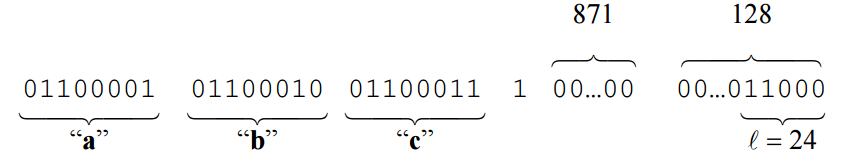
\includegraphics[width=2.5in]{padding}
\caption{An example of the SHA-256 padding}
\label{fig:pad}
\end{figure}


\begin{figure}[!t]
\centering
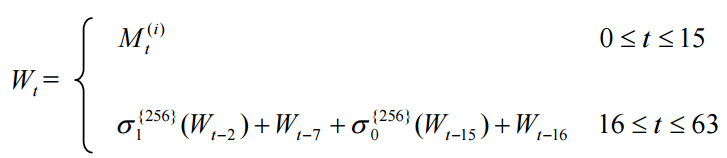
\includegraphics[width=2.5in]{messageSchedule}
\caption{The generation of the Message Schedule vector (W) based on the input Message (M)}
\label{fig:messageSchedule}
\end{figure}

\begin{figure}[!t]
\centering
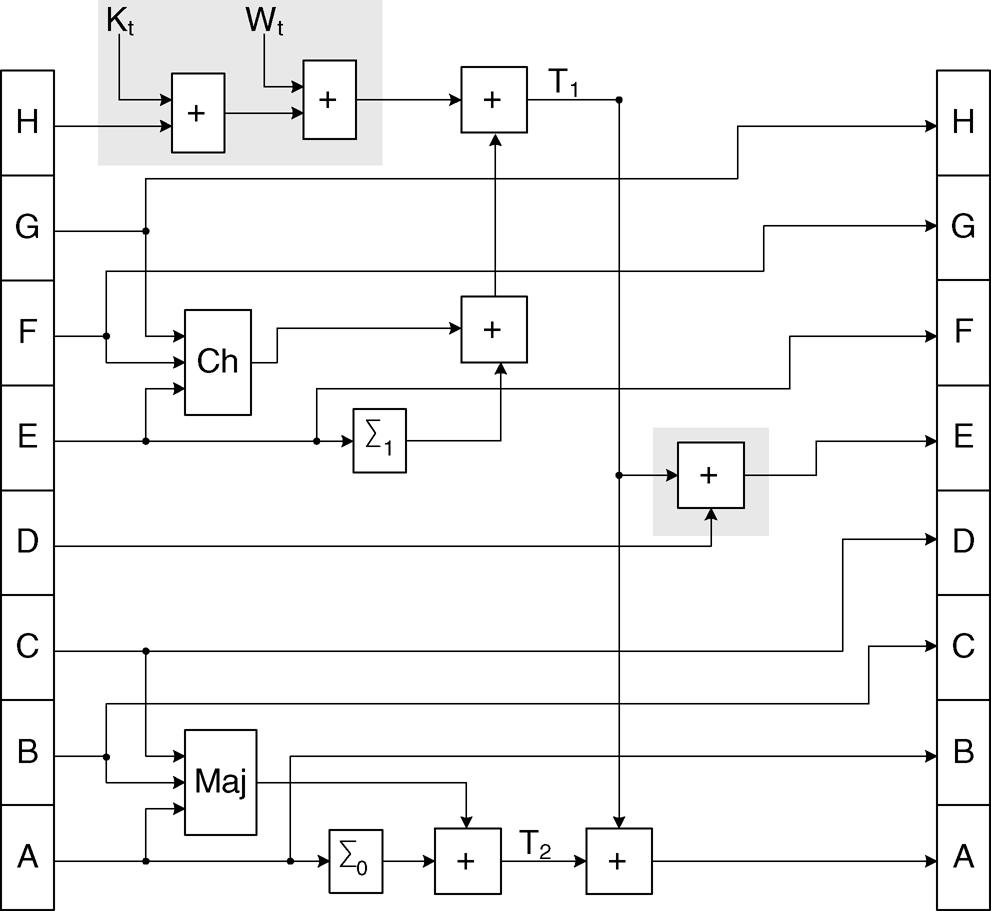
\includegraphics[width=2.5in]{sha2round}
\caption{One round of the inner loop of the SHA-256 algorithm}
\label{fig:innerloop}
\end{figure}



\section{Implementation of the SHA-2 Hash Family Standard Using FPGAs} \label{sha2fam}
The proposed architecture by Sklavos et al. \cite{sklav} supports three hash functions (256, 384 and 512) of the SHA-2 standard. Their design is aimed at reducing processing delays for networked devices such as cellphones. The proposed design boasts higher operation frequency, needs less silicon area resources than previous solutions and has a throughput 417\% faster than research at the time. What makes this system fast is their:
\begin{itemize}
\item inner loop computation
\item Data initialization block
\item ROM Stored constants 
\end{itemize}
Their solution reuses hardware cleverly because performs 32-bit operations and 64-bit operations on the same hardware. To do so they used a 64-bit buffer which they mask with zeroes during 32-bit computations. A High level overview of their solution can be seen in figure \ref{fig:archsklav}. 

\begin{figure}[!t]
\centering
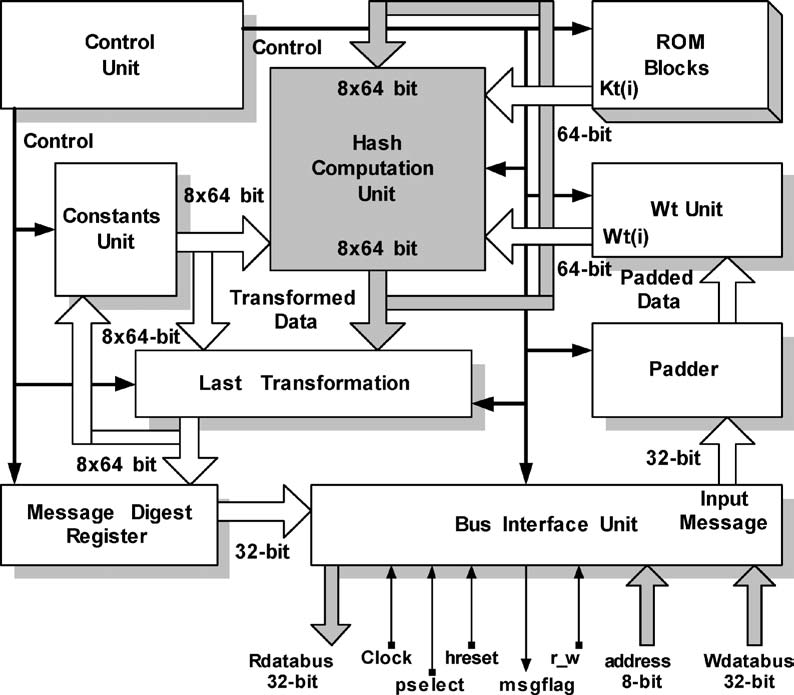
\includegraphics[width=2.5in]{archsklav}
\caption{System overview of the Sklavos et al. architecture}
\label{fig:archsklav}
\end{figure}

\subsection{Inner loop}
The inner loop computation is simple. However, the key is that they save on hardware resources by reusing the same elements for three  different algorithms. All three algorithms are similar in their inner loop or round computation but differ in the constants used for each algorithm. To get around this, they have made the sigma calculations parametrized. Figure \ref{fig:t1t2sklav} shows how each function S(n) takes in a parameter K or G depending on the algorithm.

\begin{figure}[!t]
\centering
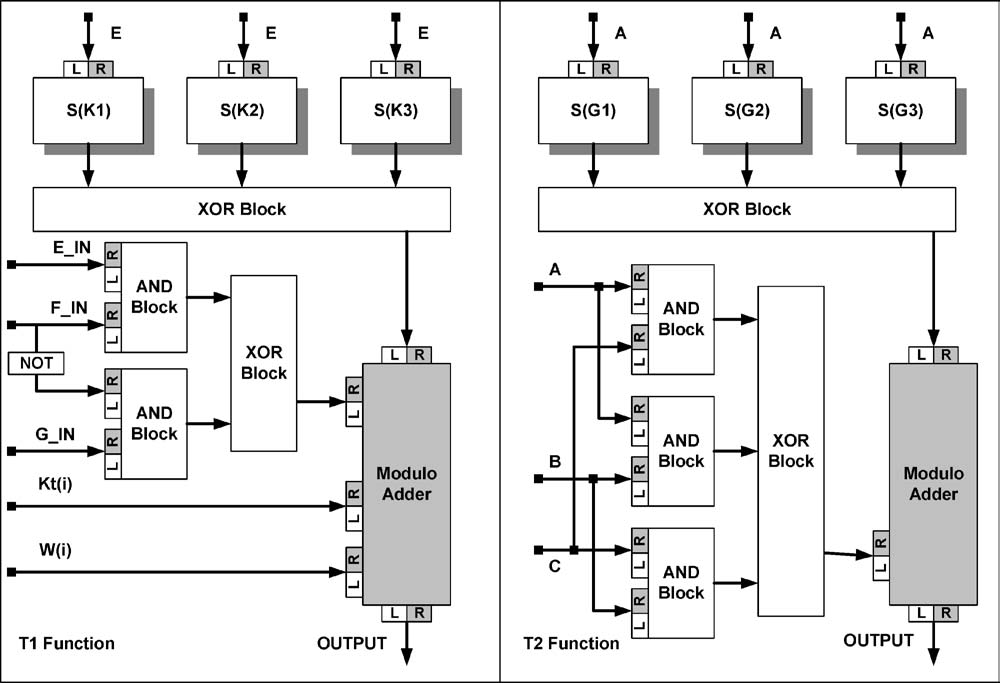
\includegraphics[width=2.5in]{t1t2sklav}
\caption{The T1 and T2 computation	}
\label{fig:t1t2sklav}
\end{figure}

\subsection{Data Initialization}
The data initialization block is made faster due to pipelining and flexible due to parametrization. Figure \ref{fig:dbesklav} shows this data initialization block. When calculating $W_t$ values for the SHA-256 algorithm, the first 16 values are straight from the message and the rest are computed from previous $W_t$ values making this step ideal for pipelining. Pipelining is used to compute the sigma values in previous clock cycles. Also, the S(n) and R(n) functions are parameterized for variables J and L depending on the algorithm, thus saving on hardware. Moreover, to speed up the lookup for constants, they've stored the constants for all three algorithms in ROM which speeds up their lookup.

\begin{figure}[!t]
\centering
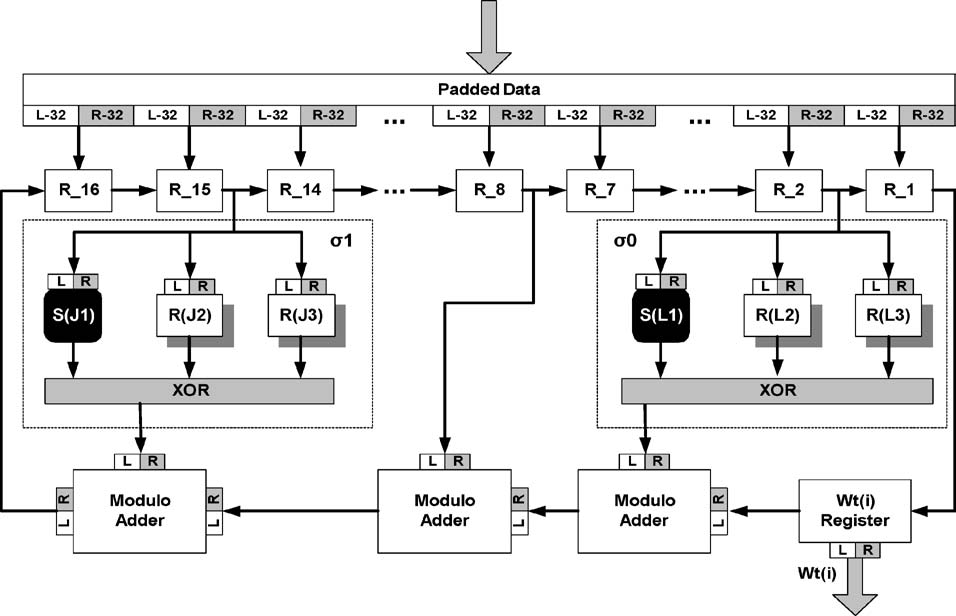
\includegraphics[width=2.5in]{dbesklav}
\caption{The data expansion block }
\label{fig:dbesklav}
\end{figure}

\subsection{Results}
The authors have taken their design and implemented on XILINX Virtex v200pq240 FPGA. These results can be seen in figure \ref{fig:compsklav}. The FPGA implementation used 2384 Configurable Logic Blocks (CLB) and achieved a throughput of 291 Mbps, 350 Mbps and 467 Mbps for SHA-256, SHA-384 and SHA-512 respectively. It is interesting to note that the throughput increases for each algorithm, this is because each algorithm is processing more data in parallel. Moreover, the architecture by Sklavos et al. achieves a higher data rate than other implementations of SHA-256. Simulations showed that the power consumption can be as low as 46mW.

\begin{figure}[!t]
\centering
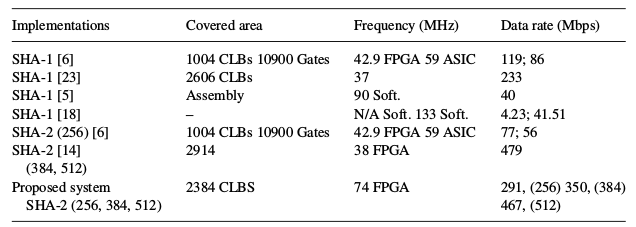
\includegraphics[width=2.5in]{compsklav}
\caption{Results comparison in the Sklavos et al. implementation}
\label{fig:compsklav}
\end{figure}

\subsection{Comments}
This research implementation demonstrates that high data rates are possible for the SHA2 hash algorithms family. However, there are some drawbacks to their work. First, the comparison made between their SHA-256 implementation and the one in \cite{md4} is not completely fair. The previous work they compare to, also computes other hash algorithms from the MD4 family. It is understandable that it is slower given that it is more flexible. Second, their introduction motivates creating faster hardware for cryptography in phones, however, their solution remains at the FPGA implementation. It would have been interesting to know if this design will scale down to the power and area requirements for the mobile applications.


\section{Cost-Efficient SHA Hardware Accelerators} \label{cesha}
The research by Chaves \cite{ceshar} improves the SHA256 computation throughput and uses less area when compared to the previous implementations in the literature and in use by the industry and 150 times speed up against pure software implementations \cite{ceshar}.  Implementation results on several FPGA technologies of the proposed SHA, show that a throughput of 1.4 Gbit/s is achievable for the SHA-256 hash functions \ref{ceshar}. To evaluate both these parameters they focus on the metric throughput per slice which is a ratio of the input bits processing speed versus the area used. Their improvements required them to carefully examined the algorithm for hotspots that can be improved and came up with three techniques to speed up the operations:
\begin{itemize}
\item operation rescheduling
\item hardware reuse
\item memory-based block expansion structures.
\end{itemize}	
The full design by Chaves et al. can be seen in figure \ref{sha256ceshar}.

\section{SHA-256 algorithm} \label{sha256}
\begin{figure}[!t]
\centering
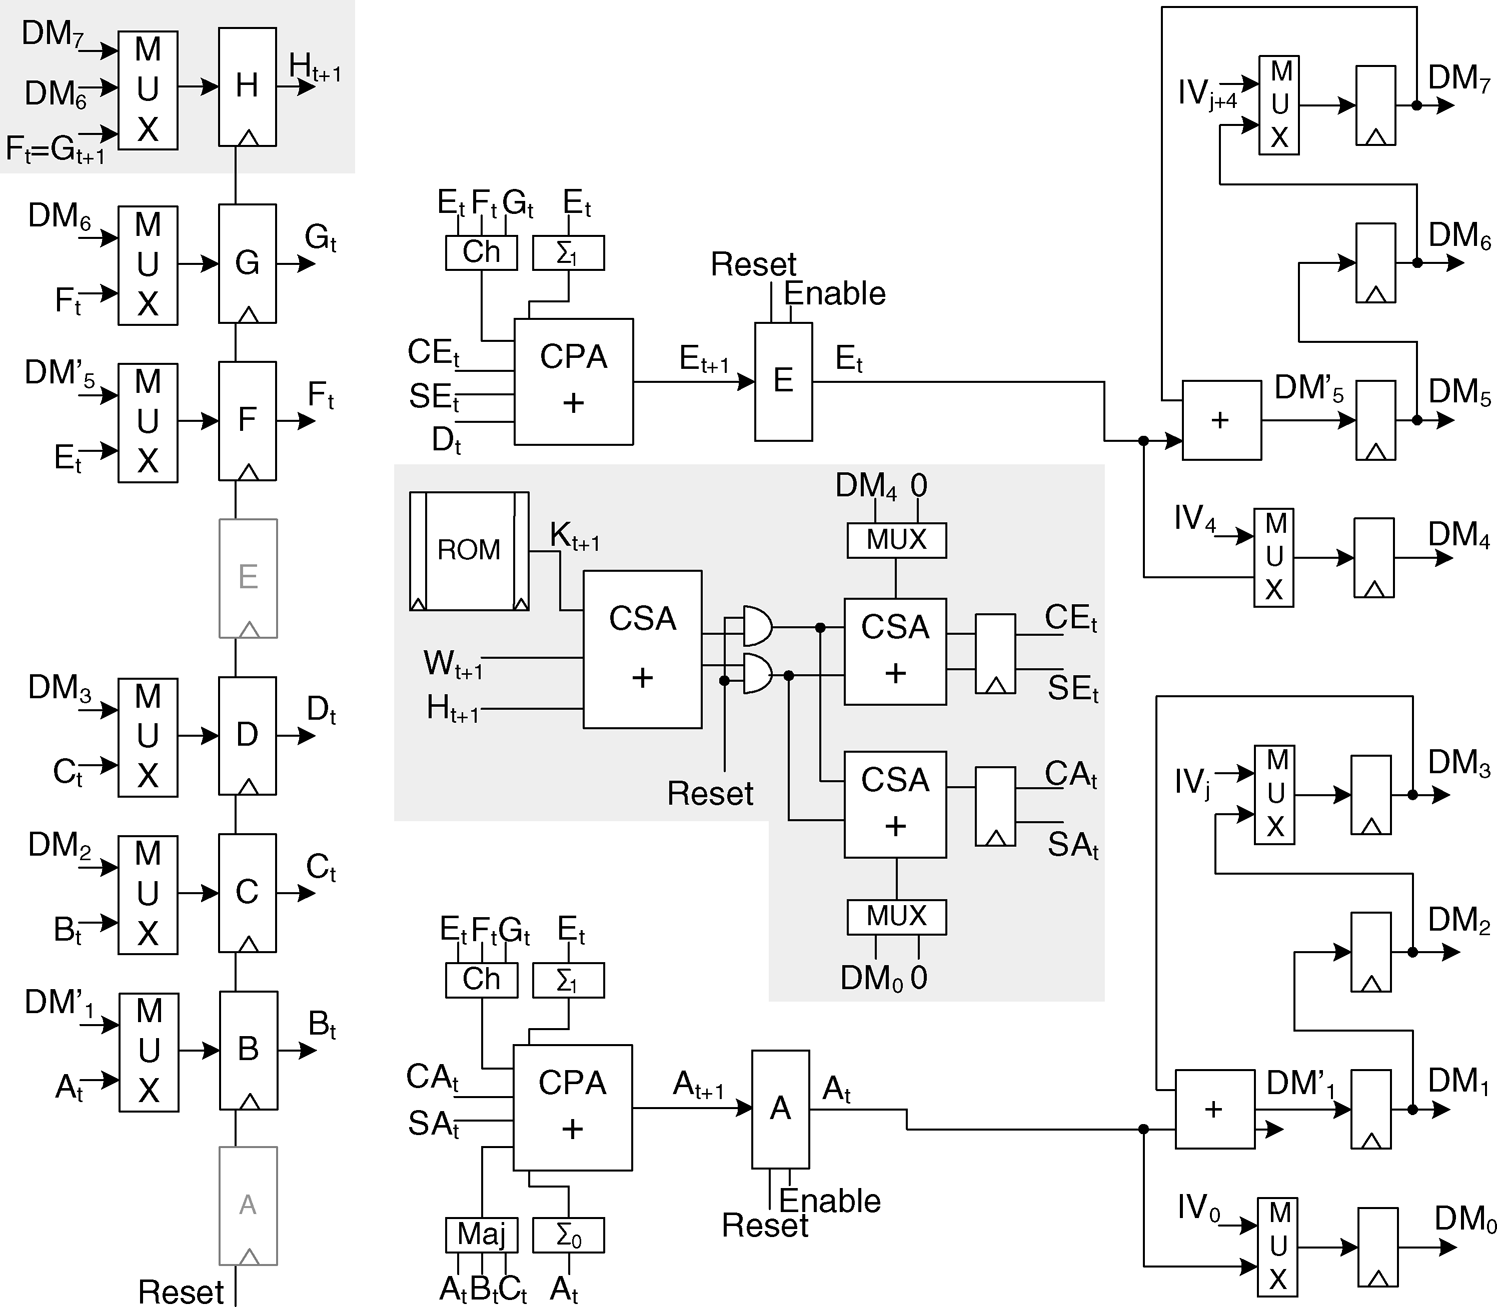
\includegraphics[width=2.5in]{sha256ceshar}
\caption{Full design of Chaves et al.}
\label{fig:sha256ceshar}
\end{figure}

\subsection{Operation rescheduling}

The technique of operation rescheduling reduces the critical path in the computation of the inner loop of the SHA-256 algorithm. The computation of A and E in the inner loop of SHA-256, as seen in figure \ref{fig:innerloop}, require the most amount of time whereas the other buffers only require a shifting operation. The computations of calculating A and E are described in \ref{fig:compAH}. To reduce the critical path of one round, the additions of H, $K_{t}$ and $W_{t}$ will happen in a previous round. This computation is described in figure \ref{fig:compAHdelta}. This results E having a critical path of 4 additions to 3 additions. 

\begin{figure}[!t]
\centering
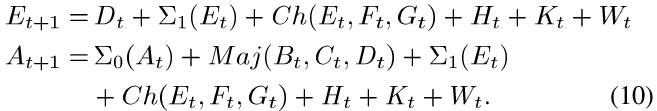
\includegraphics[width=2.5in]{eq10ceshar}
\caption{Computation of A and H}
\label{fig:compAH}
\end{figure}

\begin{figure}[!t]
\centering
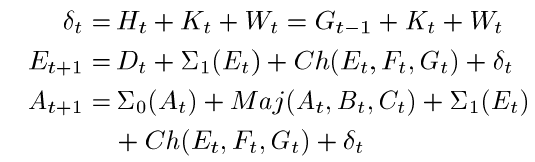
\includegraphics[width=2.5in]{eq11ceshar}
\caption{Computation of A and H with delta}
\label{fig:compAHdelta}
\end{figure}

\subsection{Hardware Reuse}
Knowing that the calculation of the new DM at the end of a block uses delayed values of A and E, it is possible to reduce the number of adders needed to calculate the output of the new DM. The relationship between the buffer variables are given in figure \ref{fig:relAH}. Thus the DM can be computed from delayed values of A and E as seen in figure \ref{fig:dmah}. Which means using only four time steps and 2 adders we can compute the values of DM as seen in figure \ref{fig:twoadd}. This technique makes the design more area efficient.

\begin{figure}[!t]
\centering
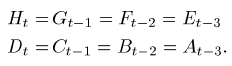
\includegraphics[width=1.5in]{eq12ceshar}
\caption{Relation between buffer variables}
\label{fig:relAH}
\end{figure}

\begin{figure}[!t]
\centering
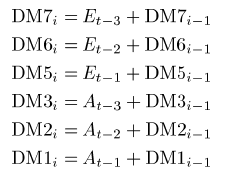
\includegraphics[width=1.5in]{eq13ceshar}
\caption{Relation between DM and A,E}
\label{fig:dmah}
\end{figure}

\begin{figure}[!t]
\centering
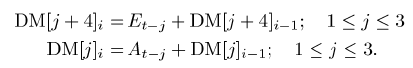
\includegraphics[width=2.5in]{eq14ceshar}
\caption{Only two adders are needed}
\label{fig:twoadd}
\end{figure}


\subsection{Data Block Initialization}
To efficiently compute the values of $W_{t}$ a datablock initialization unit is proposed and can be seen in figure \ref{fig:dbeceshar}. This also has the effect of reducing the critical path since additions are computed over several past iterations.

\begin{figure}[!t]
\centering
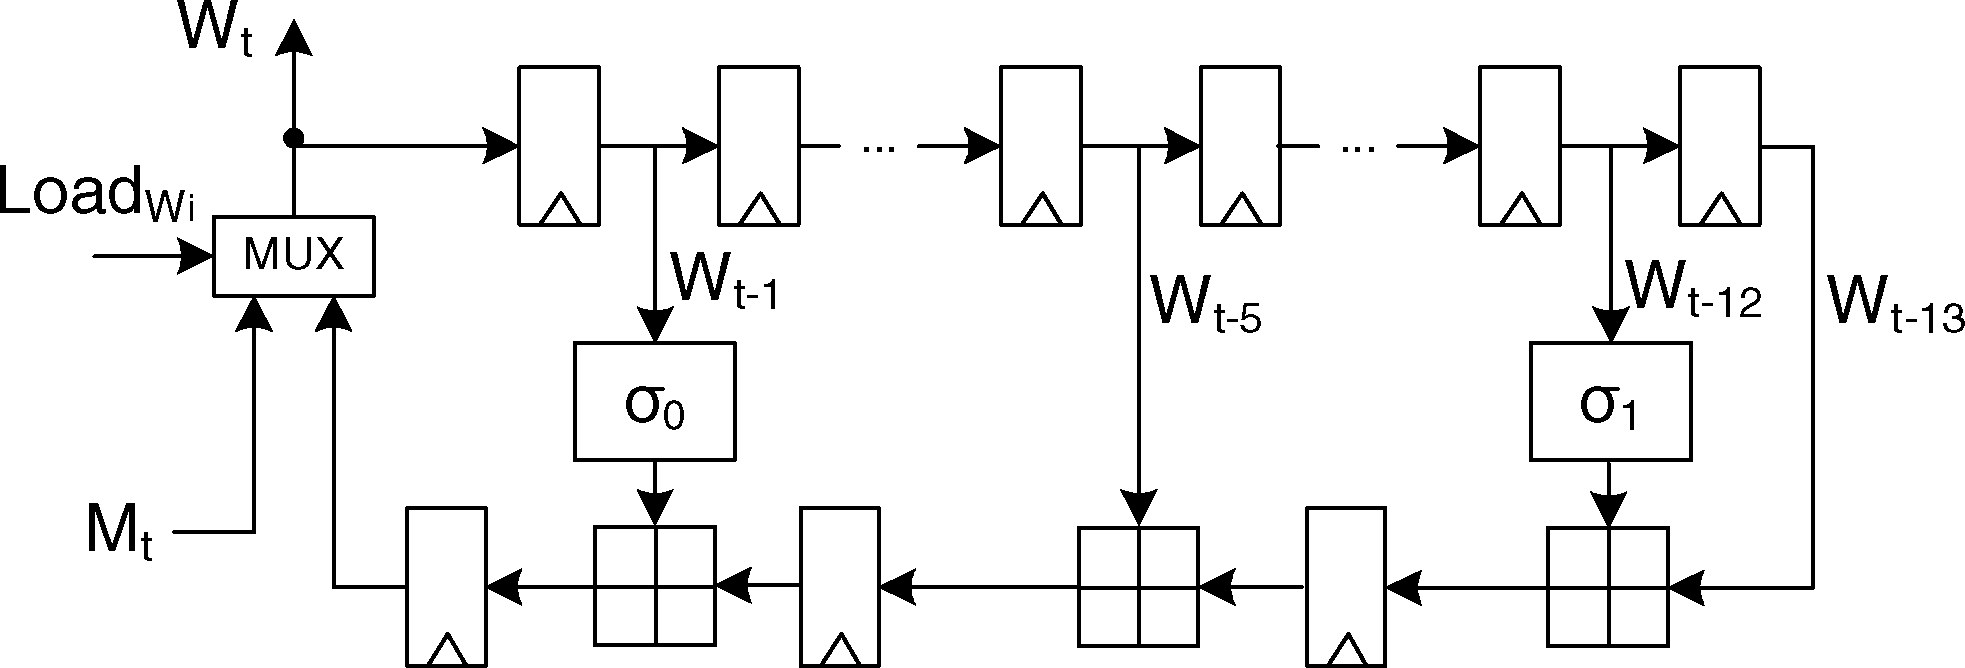
\includegraphics[width=2.5in]{datablockexpceshar}
\caption{Only two adders are needed}
\label{fig:dbeceshar}
\end{figure}



\subsection{Results}
To analyze the performance of this design, the authors have implemented their design on an VIRTEX II Pro FPGA. The comparison between other implementations can be seen in figure \ref{fig:tableceshar}. This implementation out performs both the academic implementations as well as the industry implementation. The Chaves implementation consistently has a higher throughput and lower area.
\begin{figure}[!t]
\centering
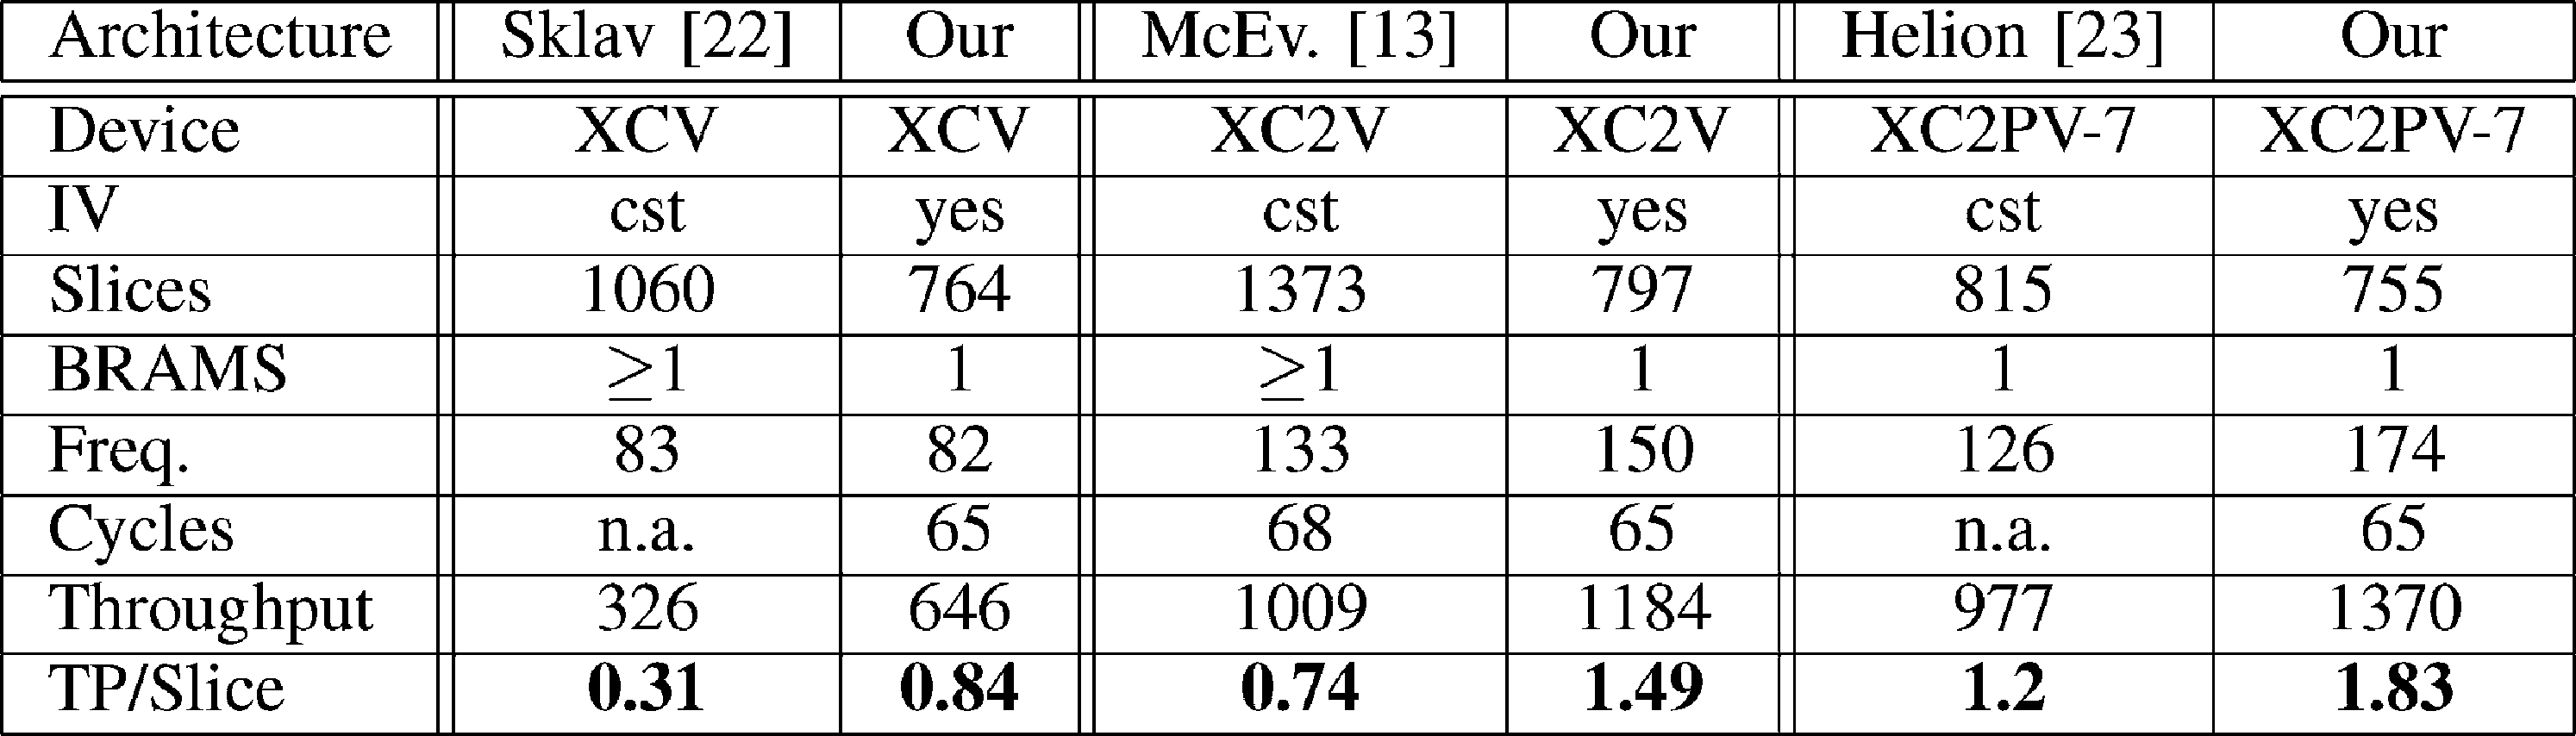
\includegraphics[width=2.5in]{tableceshar}
\caption{Only two adders are needed}
\label{fig:tableceshar}
\end{figure}


\subsection{Comments}
This paper introduces a new implementation to perform the SHA-256 algorithm. However, there are still some questions left unanswered.\\ First, there was no comparison of Data block expansion structures. The paper proposed three structures to perform Data Block expansion and ruled out 2 due to the fact that some components were not widely available on all FPGAs. Although that may be true, it would have been useful to know what the trade offs are for using the different structures in terms of throughput for designers with access to the right FPGA. \\Second, the authors show only a performance analysis of the entire system. How much did each technique contribute to speed up the algorithm or save on area? A breakdown would illustrate the impact each technique and the trade offs of including it or not. \\Third, a comparison with the Sklav implementation is not really a fair comparison. This is because the Sklav model is a flexible design that can perform three different types of SHA hashes. The throughput and area considerations for the Sklav design are impacted because of its flexibility.\\Lastly, the authors did not explain what benchmark they used to obtain their throughput results. It would have been interesting to know how to reproduce the results.


\section{On the Exploitation of a High-Throughput SHA-256 FPGA Design for HMAC} \label{Explsha}
The solution my Michail et al. \cite{michail} is the fastest in the literature. They survey the past literature notice that techniques such as retiming, pre-computation, loop unrolling etc. are used separately to improve the algorithm efficiency. Their results are achieved by using all of the previously mentioned techniques together and then some of their own. The resulting implementation has a tremendous throughput of 11Gbps after place and route on a Xilinx Virtex 6 board. This section will discuss only the unique aspects of this design.

\subsection{Loop Unrolling}
In order to speed up computation the authors of \cite{michail} used loop unrolling. Figure \ref{fig:loopunrolling} depicts the unrolling of the inner loop. The inner loop is unrolled twice to obtain a mega block. A choice of two unrolling was chosen based on a previous study that found two unrolling resulted in the best overall throughput and area performance.

\begin{figure}[!t]
\centering
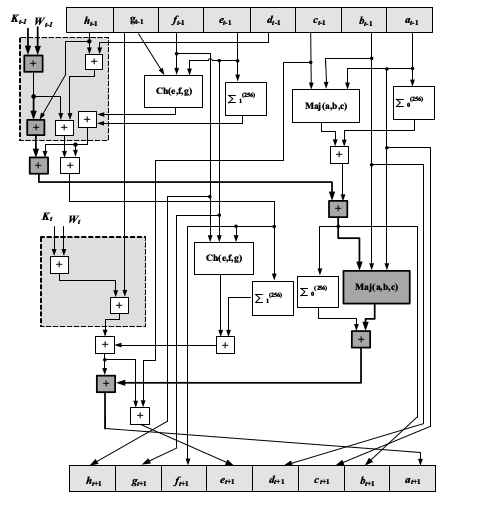
\includegraphics[width=2.5in]{loopunrolling}
\caption{Only two adders are needed}
\label{fig:loopunrolling}
\end{figure}


\subsection{Pipelining}
In this study a four stage pipeline was used in order to maximize throughput. By pipelining the round computation, the authors of \cite{michail} were able to compute four different hash values at once. This has the effect of almost quadrupling throughput. Again, 4 stages were chosen because it was the optimal throughput versus area optimization.  

\begin{figure}[!t]
\centering
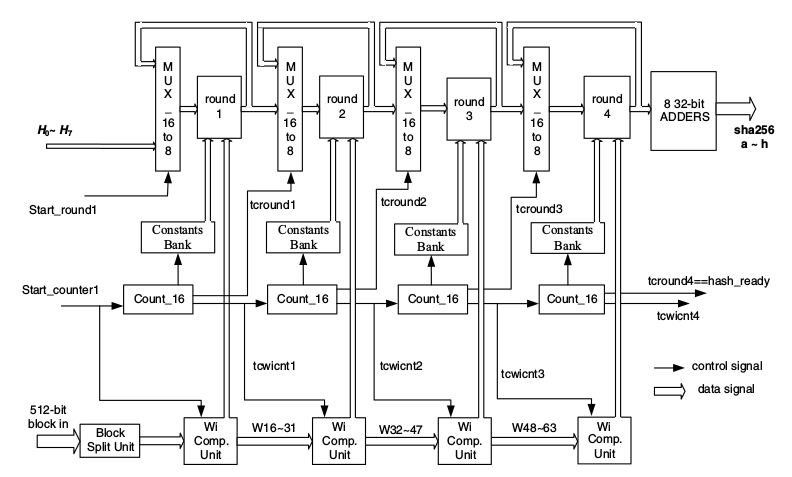
\includegraphics[width=2.5in]{archmic}
\caption{Four stage pipelining of the inner loop}
\label{fig:archmic}
\end{figure}

\subsection{Comments}
This research is a great study in the space of VLSI not only because of the amazing results in throughput but also because of the traceability of their work. Why did they choose 4 stage pipelining and not five? Why did they unroll the loop twice? Each technique had a reference to their past work justifying their techniques. However, there were no estimates of how much power it would consume. This is justified because their target application was for servers and routers which are not necessarily limited by power. 

\section{Conclusion} \label{Conclusion}
This survey is a study of three major VLSI implementations of the SHA-256 algorithm. Each adaptation improved from their predecessors to provide higher throughput over a lower area. They did so using VLSI techniques such as retiming, pre-computation, loop unrolling and pipelining paying careful attention to the parts of the algorithm that these methods were best suited to. The highest throughput achieved was by Michail et al. with a throughput of 11Gbps. Although these implementations were fast, none of these implementations were suited to the embedded computing market. Only one design discussed the estimated power consumption but neither were specifically optimizing for a low power design suited for embedded systems. As technology moves to the internet of things, it is likely that future designs will optimize for power as well. 

% http://www.michaelshell.org/tex/ieeetran/bibtex/
\bibliographystyle{IEEEtran}
% argument is your BibTeX string definitions and bibliography database(s)
\bibliography{shabibl}


% that's all folks
\end{document}


